\section{Vorstellung des Prototypen}\label{prototyp}
Der Prototyp demonstriert, wie eine Software entsprechend der in Kapitel \ref{bmc} identifizierten Bausteine einem Fahrzeughalter bereitgestellt werden kann. Konkret wird die Bereitstellung einer Software dargestellt, mit welcher \textbf{ein Fahrzeug selbstständig ein Parkticket kaufen und anschließend zum Parkplatz fahren kann.} Zunächst wird in Kapitel 5.1 dargestellt, wie der Prototyp installiert werden kann. Im Anschluss daran wird in Kapitel 5.2 die Software Architektur des Prototypen vorgestellt. Abschließend werden die Funktionen des Prototypen vorgestellt und wie diese genutzt werden können. 

\subsection{Architektur des Prototypen}	
Abbildung \hyperref[img:basic]{13} zeigt die Grundlegende Architektur des Prototypen. Über den OEM-Server \textit{(Server)} können Softwares Heruntergeladen werden. Der \textbf{Software Applikation Manager} \textit{(SAM)}, die \textbf{Carla Simulation} und die \textbf{Mensch Maschine Schnittstelle} \textit{(MMS)} bilden gemeinsam die Repräsentation des Fahrzeugs. Die Python-basierte Carla Simulation stellt das Fahrzeug in einer Stadt dar. Dieses Fahrzeug ist die visuelle Repräsentation des Prototypen. Dies restlichen Module sind alle in Java geschrieben. Die Mensch Maschine Schnittstelle ist eine Android-Schnittstelle, auf welcher eine Version des Software Shops als App installiert ist. Über diese App können Nachrichten von dem Software Applikation Manager empfangen und verarbeitet werden. Außerdem können Nutzereingaben getätigt werden um mit dem restlichen Kompnenten des Fahrzeugs zu kommunizieren. Der Software Applikation Manager ist mit allen Modulen des Prototypen verbunden und stellt daher die zentrale Steuerungseinheit des Prototypen dar. Außerdem erfolgt die Installation und Nutzung von Software auf diesen.
\begin{figure}[!h]
	\centering
	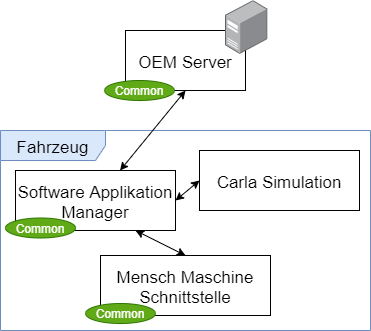
\includegraphics[width=0.5\columnwidth]{pictures/konzept-basic.png}
	\label{img:basic}
	\caption{Grundlegende Architektur der Prototypen}
\end{figure}

Der Server, SAM und die MMS kommunizieren alle auf Basis der \textbf{Common-Objekte}. Diese sind eine Sammlung an Java-Objekten, welche für die Zweckgebundene Kommunikation jedem einzelnen Modul bekannt sein muss. Sie enthalten Primitive Werte \textit{(Integer, String, Long, etc.)} und leiten alle vom Serializable-Interface ab. Abbildung \hyperref[img:common]{14} stellt die generelle Aufteilung der Objekte in zwei Gruppen dar. \\

\textbf{Environment-Objekte} sind Objekte, welche zur Umwelt des Prototypen gehören. Damit der Server spezifische Softwares verschicken kann, wird ihm die abstrakte Klasse Software zur Verfügung gestellt als auch eine Sammlung von Softwares. Jede Software des Prototypen benötigt eine eindeutige ID und eine Methode \textit{handleMessage()}, welche bestimme Messages bearbeiten kann. Auch der Software Applikation Manager nutzt diese Objekte, um so die Softwares \textit{installieren und nutzen} zu können. Die Description wird genutzt, um Softwares oder Services, die im Prototypen implementiert werden zu beschreiben. Das Provider-Objekt tut eben dies für die Beschreibung das Anbieters der Software bzw. des Services. Das Angebot repräsentiert die Auswahlmöglichkeiten, die dem Fahrzeughalter beim Kauf einer Software über die MMS vorgeschlagen werden \textit{(Kauf, Leihe, Abo)}. Alle Drei Objekte werden in der MMS genutzt um das Angebot darzustellen.

\begin{figure}[!h]
	\centering
	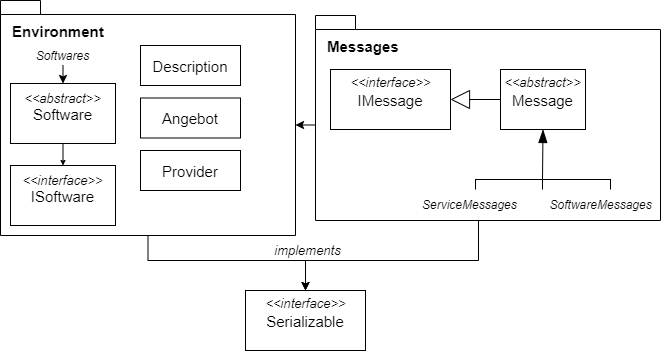
\includegraphics[width=0.8\columnwidth]{pictures/konzept-Common.png}
	\label{img:common}
	\caption{Aufbau der Common Library}
\end{figure}

Neben den Environment-Objekten gibt es auch noch Messages. Messages sind die Objekte, die im Prototypen zwischen den einzelnen Komponenten verschickt werden. Sie beinhalten neben Primitiven Datentypen auch Environment Objekte und sind ebenfalls für die zweckgebundene Kommunikation gedacht. Messages werden in SoftwareMessages oder ServiceMessages unterteilt. SoftwareMessages sind all jene Nachrichten, welche zur Installation oder Nutzung einer Software notwendig sind und ServiceMessages sind jene, die zur Nutzung eines Service notwendig sind. 

\subsubsection{Architektur des Software Applikation Managers (SAM)}
Wie zuvor erwähnt, wird über den Software Applikation Manager das Geschehen des Prototypen gesteuert. Er ist, wie in Abbildung \hyperref[img:sam]{15} zu sehen ist, in drei kleine Module aufgeteilt. In der GUI werden alle Ereignisse des Prototypen in einem Log dargestellt. Die Log-Einträge werden vom MessageHandler eingetragen. In der "Software Control Unit" baut der MessageHandler Netzwerkverbindungen zwischen sich, dem Server, der MMS und Carla auf. Jede eingehende Nachricht wird von ihm empfangen und verarbeitet. In diesem Kontext, kann eine eingegangene Nachricht an das MMS weitergeleitet werden oder es wird auf eine Nutzereingabe in der GUI gewartet. Außerdem beinhaltet der Messagehandler den SoftwareManager. Dieser verwaltet die auf dem "Fahrzeug" installierten Softwares und stellt diese zur Verfügung wenn sie zur Auswertung einer Nachricht benötigt werden.
\begin{figure}[!h]
	\centering
	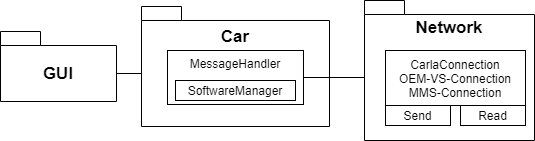
\includegraphics[width=0.8\columnwidth]{pictures/konzept-SAM.png}
	\label{img:sam}
	\caption{Architektur des Software Applikation Managers}
\end{figure}

\subsubsection{Architektur des OEM-Servers (Server)}
Die Architektur und auch die Funktionalität des Servers wurden unter der Beachtung des Uptane Standards geplant und implementiert. Die Architektur ist in Abbildung \hyperref[img:server]{16} dargestellt. Der Kern des Servers ist der \textbf{Director}, welcher eingehende Anfragen für Softwares abarbeitet. Der Director ist mit dem\textbf{ Image Repository} verbunden, in welchem sich die Softwares befinden, welche im Shop bereits bereitgestellt werden. Uptane gibt vor, eine \textbf{Inventory Database} zu führen, in welcher die Manifeste aller im Shop registrierter Fahrzeuge in der Form gespeichert sind, in welcher sie zuletzt von dem Director verifiziert wurden. Wird eine Anfrage an den Server geschickt, enthält diese das aktuelle Manifest des Fahrzeugs. Der Director vergleicht dieses mit dem Manifest, welches in der Inventory Database gespeichert ist. Durch den Vergleich des ByteCodes beider kann festgestellt werden, ob am Fahrzeug Änderungen von einer externen Instanz getätigt wurden oder nicht.
\begin{figure}[!h]
	\centering
	\includegraphics[width=0.75\columnwidth]{pictures/konzept-OEM-vs.png}
	\label{img:server}
	\caption{Architektur des Software Applikation Managers}
\end{figure}

%Abhängig von prototyp-version
Der Director kann eingehende Anfragen an den Software-User-Pattern-Recognizer\textit{(SUPR)} weiterleiten, welcher in Kapitel \hyperref[fs]{zwei} vorgestellt wurde. Der SUPR ist dafür zuständig, den Software-Bedarf von Fahrzeughaltern anhand ihrer Fahrdaten zu identifizieren. Er hat Zugriff auf das Image Repository und das \textit{Scenario Repository}. In diesem werden, wie in Kapitel \hyperref[konzept]{zwei} erwähnt, die zu einer Software hinzugefügten Szenarien gespeichert. Der Director leitet Anfragen weiter, die das feststellen von Softwarebedarf umfassen. Er selber verarbeitet nur die direkten Kaufanfragen für Software.

\subsection{Installation}
Die Installation der einzelnen Module muss muss getrennt voneinander passieren. Für die vollständige Nutzung muss sichergestellt sein, dass Carla auf dem PC auf welchem der Prototyp installiert werden soll lauffähig ist. Schauen Sie sich hierzu die Systemanforderungen von Carla an.\footnote{Carla Systemanforderungen} Die einzelnen Module können auch auf getrennten Geräten genutzt werden, indem die IP-Adressen und Ports der Module über deren Config-Dateien angepasst werden. Die folgende Anleitung stellt dar, welche Schritte zur Installation der einzelnen Module getätigt werden müssen. Sie ist für Windowsgeräte ausgelegt und dauert ca. \\
\\
\textbf{ZEIT EINFÜGEN Minuten}


\subsubsection{Server und SAM Installation}
\begin{itemize}
	\item[\textbf{1.}] \textbf{.zip-Ordner Herunterladen}\\
	Gehen Sie auf \url{https://github.com/hesty98/bachelorthesis}. Klicken Sie auf den \textit{"releases"}-Tab, welcher unter der Beschreibung des Repository zu finden ist.
	Laden Sie die Datei \textit{"prototyp.zip"} herunter und entpacken Sie den Ordner auf ihrem Laptop. In diesem Ordner finden Sie die .jar-Dateien mit welchen der Server und der SAM gestartet werden können. Der Ordner \textit{"PythonScriptsThesis"} wird später für die Installation von Carla benötigt.
	
	\item[\textbf{2.}] \textbf{IP-Adresse aufschreiben}\\
	Um das MMS und auch Carla mit dem Software Applikation Manager zu verbinden, müssen Sie ihre IP-Adresse kennen. Öffnen Sie hierzu ihr Windows-Temrinal und geben Sie \textit{ipconfig} ein. In der Zeile "IPv4-Adresse" steht ihre die IP-Adresse. Diese müssen Sie sich merken.
\end{itemize}


\subsubsection{MMS Installation}
\begin{itemize}
	\item[\textbf{1.}] \textbf{Android Studio herunterladen}\\
	Sie haben zwei Optionen, wie die Mensch Maschine Schnittstelle genutzt werden kann. Entweder sie simulieren das Android Gerät auf ihrem PC oder Sie installieren die App auf ein eigenes Tablett/Smartphone. Für beides wird eine aktuelle Version von Android Studio benötigt, die Sie hier \url{https://developer.android.com/studio} herunterladen können. Installieren Sie Android Studio und fahren Sie anschließend vor.

	\item[\textbf{2.}] \textbf{Code importieren}\\
	Das Repository der Mensch Maschine Schnittstelle liegt auf GitHub. Über Android Studio können Sie das Projekt direkt importieren. Klicken Sie hierfür auf "File" -> "new" -> "Project from Version control" -> "GitHub" und geben sie folgende URL ein: \url{https://github.com/hesty98/HMI}.\\
	
	\textbf{TESTEN}\\
	
	Alternativ kann das Projekt auch als .zip-Datei Heruntergeladen werden. Der extrahierte Ordner kann in Android Studio als Projekt geöffnet werden \textit{(File -> open -> Ordner wählen)}.
	
	\item[\textbf{3.}] \textbf{MMS Konfigurieren}\\
	Öffnen Sie in Android Studio die Datei Connection.java und passen Sie den Host entsprechend der IP des \textit{Software Applikation Managers} an. Die Datei befindet sich im 'network'-Ordner \textit{(app -> java -> com.linushestermeyer.hmi -> network)}.
	
	\item[\textbf{4.}] \textbf{MMS aufsetzen}\\
	Sie können die Mensch Maschine Schnittstelle nun entweder auf einem eigenen Gerät installieren oder das Gerät auf ihrem PC simulieren. Für beide Optionen Sie zuerst eine Konfiguration für die App erstellen.  Folgen Sie hierzu folgender Anleitung: \url{https://developer.android.com/studio/run/rundebugconfig}.
	
		\subitem \textbf{4.1 Eigenes Tablet}\\
			Zur Installation auf ihrem Tablet müssen Sie zunächst die \textit{Entwickler-Optionen} für dieses Freischalten und \textit{USB-Debugging} aktivieren. Folgen sie hierfür folgender Anleitung: \url{https://mobilsicher.de/ratgeber/usb-debugging-aktivieren}. Wurde dies getan, kann das Gerät an den PC angeschlossen werden. Über den grünen 'Play'-Button in der oberen Menuleiste kann die App auf Ihrem Gerät installiert werden.
			
		\subitem \textbf{4.2 Virtual Device}\\
			Wenn Sie Die App \textbf{nicht} auf einem eigenen Gerät installieren wollen, müssen sie mit Android Studio ein Simuliertes Gerät erstellen. Dies funktioniert nur, wenn ihr PC eine \textbf{Intel-CPU} hat, da Android Studio den \textit{HAXM-Service} von Intel zur Simulation nutzt. Verfügt ihr PC über eine Intel-CPUD, können Sie mit Hilfe folgender Anleitung ein Virtuelles Gerät erstelle: \url{https://developer.android.com/studio/run/managing-avds}. Erstellen Sie eine Instanz eines Tablets, nicht die eines Smartphone. \\
			Haben Sie ein \textit{VD} erstellt, können sie anschließend über den grünen 'Play'-Button in der oberen Menuleiste die App auf diesem Gerät installieren. 
\end{itemize}


\subsubsection{Carla Installation}
\begin{itemize}
	\item[\textbf{1.}] \textbf{Python installieren und SYS\_PATH hinzufügen}\\
	Damit Carla auf dem PC laufen kann, muss Python in Version 3.7 auf dem PC installiert sein und dem SYSTEM\_PATH hinzugefügt werden. Hierzu kann folgende Anleitung genutzt werden: \url{https://geek-university.com/python/add-python-to-the-windows-path/}. Hier die 3.4 nur durch eine 3.7 gedanklich ersetzen. Der PATH kann by der Installation auch durch das ankruezen einer Checkbox automatisiert werden.
	
	\item[\textbf{2.}] \textbf{Carla Herunterladen}\\
	Carla kann als .zip-Ordner Heruntergeladen werden. Die Dateien müssen in einen eigenen Ordner auf dem PC extrahiert werden. Als nächstes öffnen sie den Speicherort von Carla im Explorer und öffnen in diesem Fenster das Terminal \textit{(geben sie 'cmd' in den Suchbalken des Explorers ein)}. Jetzt müssen die für die Simulation notwendigen  Python-Packages \textit{pip, pygame und numpy} installiert werden. Die pip-Installation kann hier nachgelesen werden: \url{https://pypi.org/project/pip/}. Für die Installation von pip sollte zudem eine Adminsitrator-Konsole verwendet werden \textit{(Windows -> suche cmd' -> 'Als Administrator öffnen')}.Ist pip installiert, können mittels folgender Zeile die übrigen packages hinzugefügt werden:
	\begin{verbatim}
	py -3.7 -u pip install --user pygame numpy 
	EINFÜGEN HILFE
	\end{verbatim}
	Im Anschluss daran sollten Sie Carla ein mal testen. Starten Sie zunächst die Carla.exe und wechseln sie im Terminall in den PythonAPI/examples Ordner \textit{(cd PythonAPI/examples)}. Führen Sie anschließend folgenden Befehl durch:
	\begin{verbatim}
	py- 3.7 spawn_npc.py
	\end{verbatim}
	\item[\textbf{3.}] \textbf{Skripte einfügen}\\
	In der extrahierten .zip-Datei des SAM und Servers befindet sich ein Ordner mit dem Namen \textit{PythonScriptsThesis}. Kopieren Sie diesen Ordner in den \textit{PythonAPI}-Ordner von Carla und Sie haben es geschafft! 
	\item[\textbf{4.}] \textbf{Carla Konfigurieren}\\
	Abschließend sollten sie noch Konfigurationen an Carla vornehmen. Zuerst wird die Stadt geändert in welcher sich das Szenario abspielen wird. Hierzu\\
	\textbf{EINFÜGEN}\\
	
	Haben Sie die entsprechenden Werte eingetragen, speichern und schließen Sie die Datei. Anschließend wechseln sie in den Ordner \textit{PythonAPI/PythonScriptsThesis} und editieren Sie die install\_sw\_use\_service.py. Passen Sie die IP an die des \textbf{Software Applikation Managers} an. 
\end{itemize}

\subsection{Nutzung des Prototypen}
Die Module des Prototypen müssen in bestimmter Reihenfolge gestartet werden:
\begin{itemize}
	\item[\textbf{1.}]\textbf{Server}\\
	Server.jar ausführen.
	\item[\textbf{2.}]\textbf{Software Applikation Manager\\}
	SAM.jar ausführen
	\item[\textbf{3.}]\textbf{Carla\\}
	Starten Sie Carla. Führen Sie anschließend im Terminal im Ordner \textit{"PythonAPI/PythonScriptsThesis"} das Skript install\_sw\_use\_service.py aus.
	\begin{verbatim}
	py -3.7 install_sw_use_service.py
	\end{verbatim} 
	\item[\textbf{4.}]\textbf{Mensch Maschine Schnittstelle}\\
	Starten Sie die App auf ihrem Gerät oder in dem Virtual Device. Gehen Sie sicher, dass die App zuvor geschlossen war.
\end{itemize}
Im folgenden haben Sie fünf Bildschirme, über die alle Module des Prototypen sichtbar sind. Die Mensch Maschine Schnittstelle wartet auf eingehende Nachrichten, ebenfalls wie Carla. Die GUI des Software Applikation Managers ist in drei Bereiche aufgeteilt. Der Log auf Linken Seite stellt alle Ereignisse aus Sicht des Fahrzeugs dar. Der Log auf der Rechten Seite der GUI stellt sämtliche Ereignisse dar, die von dem Parkautomaten wahrgenommen werden. Zwischen beiden Logs sind diverse Knöpfe, die für die Steuerung des Prototypen gedacht sind.\\
$\underline{\textbf{Auto spawnen}}$ spawnt das Fahrzeug in der Carla Simulation. Mit den WASD-Tasten und der Maus können Sie herauszoomen und das Fahrzeug suchen. Prinzipiell ist es links vor ihnen. Der $\underline{\textbf{Zum Parkplatz fahren}}$-Knopf lässt das Fahrzeug in der Simulation zu einem Parkplatz fahren und es hält dort an.\\
Der $\underline{\textbf{In Erkennungsbereich fahren}}$-Knopf lässt das Fahrzeug in den Bereich fahren, in welchem der Parkautomat dieses erkennen kann. Nun kann sich der Parkautomat über den $\underline{\textbf{Sende Service Registrierung}}$-Knopf beim Fahrzeug registrieren. Der $\underline{\textbf{Sende ActionMessage}}$-Knopf sendet eine Nachricht an Carla, die entweder das Auto parken lässt oder es vom Parkplatz entfernen lässt. Das Szenario kann durch den $\underline{\textbf{Neustarten}}$-Knopf beliebig oft durchgeführt werden. Durch den $\underline{\textbf{Hack Car!}}$-Knopf wird das Auto "gehackt". Dies soll den Fall darstellen, wenn ein Fahrzeug versucht eine Software vom Shop zu installieren aber extern Änderungen im Auto vorgenommen wurden. Durch Änderungen am Fahrzeug verändert sich das Manifest des Fahrzeug, weshalb ein Fahrzeug keine Kommunikation mit dem Server aufbauen kann. Sämtliche Ereignisse die in Folge eines Knopfdrucks passieren, werden in den Logs notiert.\\\\
Über die \textbf{Mensch Maschine Schnittstelle} kann auf vom SAM verschickte Nachrichten reagiert werden. Initial ist der Home Screen des Shops zu sehen. Erhält das die MMS eine Software- oder ServiceRegistrationMessage, erscheint ein PopUp, in welchen der entsprechende Service bzw. die Software vorgestellt wird. Es kann entschieden werden, welches Angebot genommen werden soll oder auch die komplette Transaktion mit \textbf{Cancel} abgebrochen werden.

Die Server-GUI und die Simulation stellen weitere Visuelle Repräsentationen des Prototypen dar. In beiden können die Auswirkungen nachvollzogen werden, die durch die MMS und den SAM geschehen.

\subsection{Analyse des Prototypen und Ausblick auf die Weiterentwicklung}
Im Prototypen wurde die im Forschungsseminer erläuterte Uptane Architektur versucht grundlegend zu implementieren. Hierdurch konnte gezeigt werden, wie ein Fahrzeug in der Zukunft von externen Eingriffen geschützt werden könnte. Die erstellte Software Architektur lässt eine einfache Erweiterung des Prototypen zu. Für einen neuen Anwendungsfall muss bloß eine neue Software erstellt werden und das Carla Skript muss angepasst werden. Dies dauert ca. zwei Stunden. Die Installation des Prototypen ist relativ Zeitaufwendig und komplex, weshalb das Bereitstellen einer detaillierte Anleitung wichtig gewesen ist. \\

Der Prototyp hat dargestellt, wie eine Software über eine kabellose Schnittstelle orts- und zeitunabhängig gekauft und installiert werden kann. Zusätzlich wurde die Interaktion mit den in der Wertschöpfungskette identifizierten Service Providern implementiert, was zusätzliche Anwendungsfälle bieten kann. Über die GUIs kann nachvollzogen werden, was aktuell im Fahrzeug passiert und die Simulation kann ausreichend gesteuert werden. Die visuelle Repräsentation des Fahrzeugs in Carla unterstützt die Wirkung des Prototypen enorm, da der Betrachter direkt die Auswirkungen seiner Entscheidungen sieht. Auch die Interaktion über die Android-basierte Mensch Maschine Schnittstelle hat sich als sinnvoll erwiesen, da hierdurch ein guter Bezug zur Realität und Android Automotive gezogen werden kann. \\

Der Prototyp bietet noch eine Vielzahl an Erweiterungsmöglichkeiten. Der \textbf{Server} könnte um weitere Uptane-Funktionen erweitert werden. Die Erstellung eines Server-seitigen SUPR kann Türen öffnen, komplexe Suchalgorithmen auf der Basis von OpenScenario-Dateien in den Prototypen zu integrieren. Auch der \textbf{Software Applikation Manager} kann durch diverse neue Funktionen Sinnvoll erweitert werden. Ein Fahrzeug-basierter SUPR, dargestellt in Kapitel \ref{3.3}, kann Bestimmen von ein PopUp auf der MMS erscheinen soll und sodurch das wahllose erscheinen von PopUps verhindern. Die Steuerung über die GUI sollte den neuen Anwendungsfällen entsprechend angepasst werden, da nicht in jedem Anwendungsfall eine Kommunikation mit einem Service Provider stattfindet. Entfernt man sämtliche Nutzereingaben des Prototypen und automatisiert so die gesamte Simulation, können die dargestellten Anwendungsfälle beliebig hoch skaliert werden, wodurch ein Shop und die Zuverlässigkeit der Bereitstellung getestet werden kann.\\

Im Laufe der Entwicklung wurde deutlich, dass Carla äußerst umfangreich ist. Würden die Funktionen von Carla ausgereizt werden, könnte eine Vielzahl neuer Anwendungsfälle zum Prototypen hinzugefügt und in Carla visuell dargestellt werden. Auch eine wechsel zwischen autonomen Fahrfunktionen und eigenständiger Steuerung des Fahrzeugs kann in Carla erfolgen. Im aktuellen Prototypen ist Carla nur eine visuelle Repräsentation. Durch eine Implementierung des SAM in Python kann dies korrigiert werden und die Architektur kann um ein Modul verkleinert werden. Carla wäre dadurch sowohl die visuelle Repräsentation des Fahrzeugs als auch die "Business Logik".